\documentclass[presentation,aspectratio=43]{beamer}

\usepackage{hyperref}
\newcommand{\arxivlink}[2]{{\texttt{arXiv:\,\href{https://arxiv.org/abs/#1}{#1\,[#2]}}}}

\titlegraphic{\hfill
\includegraphics[height=1.25cm]{durham-logo}}
\usepackage{appendixnumberbeamer}
\usepackage{amsmath}
\usepackage{amssymb}
\usepackage{minted}


\DeclareMathOperator{\grad}{grad}
\let\div\relax
\DeclareMathOperator{\div}{div}
\DeclareMathOperator{\curl}{curl}
\usetheme{metropolis}
\setbeamertemplate{title graphic}{
  \vbox to 0pt {
    \vspace*{1em}
    \inserttitlegraphic%
  }%
  \nointerlineskip%
}
\metroset{background=light,progressbar=frametitle,numbering=counter,block=fill}

% https://www.dur.ac.uk/marketingandcommunications/marketing/branding/colourpalette/
% Most of these are indistinguishable to those suffering colour blindness
\definecolor{purple}{HTML}{7e317b}
\definecolor{lightpurple}{HTML}{D8ACE0}
\definecolor{blue}{HTML}{006388}
\definecolor{red}{HTML}{AA2B4A}
\definecolor{green}{HTML}{9FA161}
\definecolor{yellow}{HTML}{E8E391}
\definecolor{pink}{HTML}{C43B8E}
\definecolor{lightblue}{HTML}{C4E5FA}

\setbeamercolor{normal text}{
  fg=black,
  bg=white
}
\setbeamercolor{alerted text}{
  fg=red
}
\setbeamercolor{example text}{
  fg=blue
}

\setbeamercolor{palette primary}{%
  use=normal text,
  fg=normal text.bg,
  bg=purple,
}

\author{Lawrence Mitchell\inst{1,*} \\
  \and {\scriptsize
    P.~E.~Farrell (Oxford)
    \and
    R.~C.~Kirby (Baylor)
    \and
    M.~G.~Knepley (Buffalo)}}
\institute{
  \inst{1}Department of Computer Science, Durham University\\
  \inst{*}\texttt{lawrence.mitchell@durham.ac.uk}}

\date{February 27, 2019}
\title{A new configurable preconditioner for subspace correction methods in
  PETSc}

\graphicspath{{./\jobname.figures/}{../pictures/}}

\begin{document}

\maketitle

% \begin{abstract}
%   Small block overlapping, and non-overlapping, Schwarz methods are
%   theoretically highly attractive as multilevel smoothers for a wide
%   variety of problems that are not amenable to point relaxation
%   methods.  Examples include monolithic Vanka smoothers for Stokes,
%   overlapping vertex-patch decompositions for $H(\text{div})$ and
%   $H(\text{curl})$ problems, along with nearly incompressible
%   elasticity and augmented Lagrangian schemes.

%   While it is possible to manually program these different schemes,
%   their use in general purpose libraries has been held back by a lack
%   of generic, composable interfaces.  We present a new approach to the
%   specification and development such additive Schwarz methods in PETSc
%   that cleanly separates the topological space decomposition from the
%   discretisation and assembly of the equations.  Our preconditioner is
%   flexible enough to support overlapping and non-overlapping additive
%   Schwarz methods, and can be used to formulate line, and plane
%   smoothers, Vanka iterations, amongst others.  We illustrate these
%   new features with some examples utilising the Firedrake finite
%   element library.
% \end{abstract}

\begin{frame}
  \frametitle{Multigrid for X}
  \begin{itemize}
  \item Multigrid in H(div) and H(curl)
    \only<1>{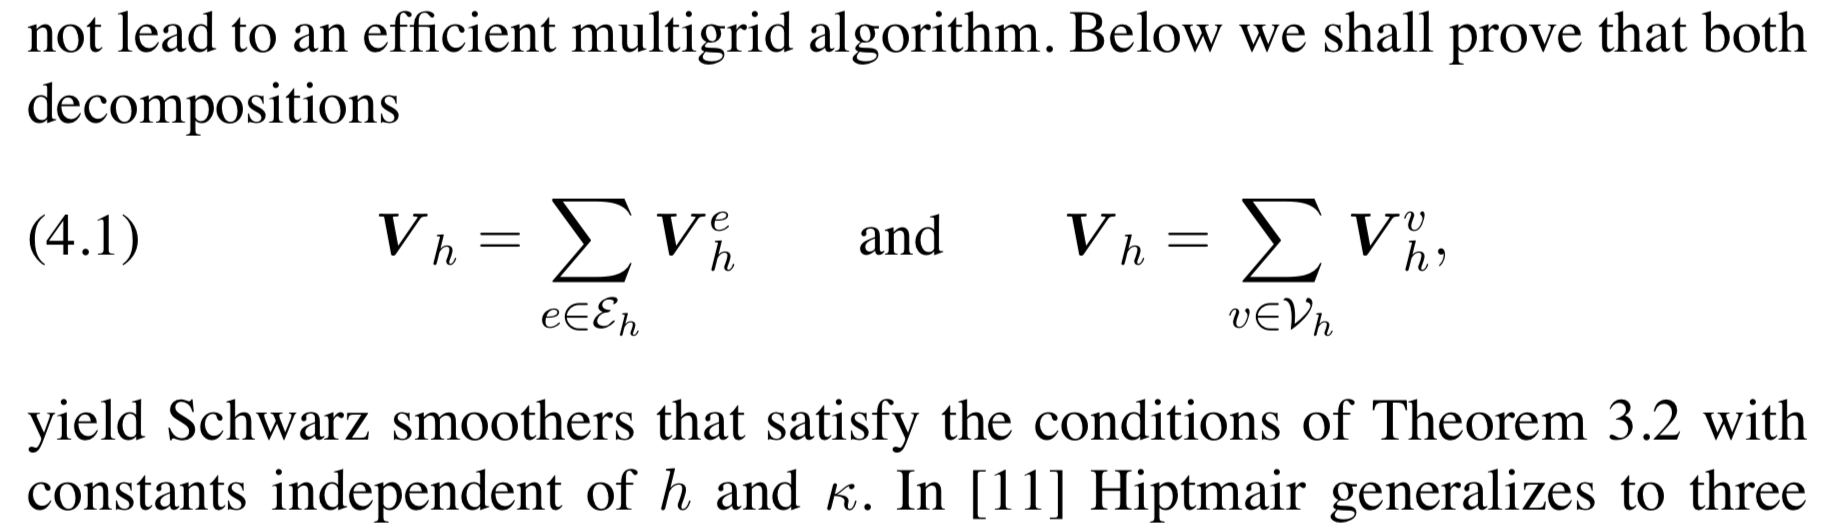
\includegraphics[width=0.8\textwidth]{hdivcurl}}
  \item Schoeberl (incompressible elasticity)
    \only<2>{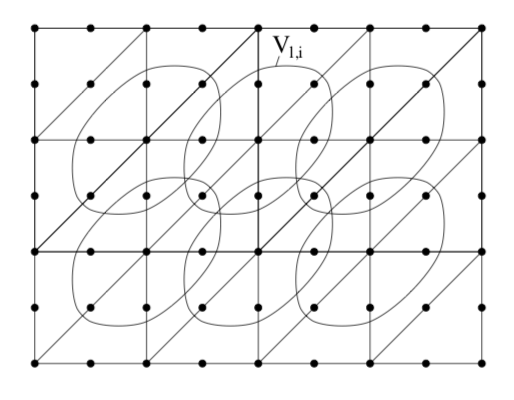
\includegraphics[width=0.5\textwidth]{elasticity}}
  \item Benzi \& Olshanskii (Navier--Stokes)
  \item Vanka (monolithic multigrid)
    \only<3>{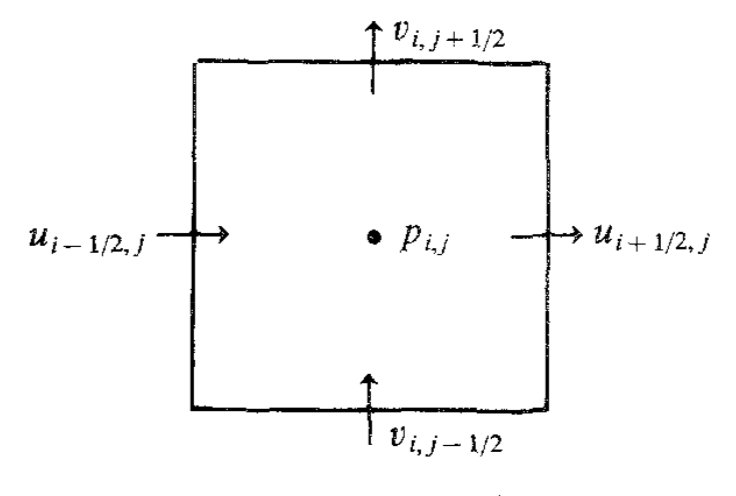
\includegraphics[width=0.8\textwidth]{vanka}}
  \item Lee et al. (Abstract convergence theory)
  \item Pavarino (Schoeberl) patch smoothers for high order H1.
  \item Line smoothing for advective problems
  \end{itemize}
\end{frame}

\begin{frame}
  \frametitle{Unifying observation}

  \begin{block}{Abstract smoother definition}
    Pick subspace decomposition
    \begin{equation*}
      V = \sum_i V_i
    \end{equation*}

    Smoother is then
    \begin{equation*}
      S = \sum_i A_i^{-1}
    \end{equation*}

    $A_i$ is defined by $(A_i x, y) = (A x, y) \, \forall x, y \in V_i$
  \end{block}

  \begin{block}{Subspace smoother}
    ... (get from Schoeberl paper?)
  \end{block}
  \begin{itemize}
  \item Decompose subspace based on topological decomposition of mesh
  \item Solve little problems based on assembly of patches
  \item Combine additively or multiplicatively
  \item Possibly (e.g. Vanka) apply some contraints in the assembly
  \end{itemize}
\end{frame}

\begin{frame}
  \frametitle{Appropriate decompositions}
  \begin{itemize}
  \item Choice of spaces determines appropriate space decomposition
  \item e.g. H(div): vertex or edge-based
  \item Vanka: (cellwise: MAC (RT0-P0)); (vertex-based: P2-P1)
  \item High order H1: vertex-based
  \item Navier--Stokes: vertex-based
  \end{itemize}
  \begin{corollary}
    Need choice to come from library that controls discretisation/PDE
  \end{corollary}
\end{frame}

\begin{frame}
  \frametitle{Configuring space decomposition: DMPlex + PetscSection}
  \begin{block}{Topological decomposition}
    DMPlex provides topological relationships:

    closure; star, etc...

    Use this to build topological patches.

    Patch is defined by set of points we are going to solve problem in
    one go on.
  \end{block}

  \begin{block}{Space decomposition}
    PetscSection attaches degrees of freedom to mesh points.

    Gather dofs to create list of patch dofs.
  \end{block}
\end{frame}

\begin{frame}
  \frametitle{Patch operator}
  \begin{itemize}
  \item If we only want homogeneous Dirichlet, can use list of dofs to
    select from assembled global operator
  \item Other transmission conditions this doesn't work
  \item Instead, callback interface
  \item Build small ``mesh'' on each patch, call back to PDE library
    to assemble operator
  \item Naturally extends to \emph{nonlinear} smoothers
  \end{itemize}
\end{frame}


\begin{frame}
  \frametitle{\texttt{-pc\_type patch}}
  \begin{itemize}
  \item DMPlex + PetscSection for subspace decomposition
  \item Callback interface to build operators
    \begin{itemize}
    \item Works if you use \texttt{PetscDS}
    \item Works with \texttt{PatchPC} in Firedrake
    \end{itemize}
  \item KSP on each patch for solves
  \end{itemize}
\end{frame}

\begin{frame}
  \frametitle{\texttt{-snes\_type patch}}
  \begin{itemize}
  \item DMPlex + PetscSection for subspace decomposition
  \item Callback interface to build operators and residual
    \begin{itemize}
    \item Not yet hooked up with \texttt{PetscDS}
    \item Works with \texttt{PatchSNES} in Firedrake
    \end{itemize}
  \item SNES on each patch for solves
  \item Enables nonlinear smoothers
  \end{itemize}
\end{frame}

\begin{frame}[fragile]
  \frametitle{Nearly incompressible elasticity}
    Find $u \in V \subset H^1$ s.t.
    \begin{equation*}
      (\grad u, grad v) + \gamma (\div u, \div v) = (f, v) \quad \forall v \in V.
    \end{equation*}

    Need subspace decompositition that spans $\ker \div$.

    Use discrete subspace of the ``Stokes complex''

    2D: $P_k$, $k \ge 4$

    ``Star'' patches around vertices

\begin{minted}[fontsize=\scriptsize]{python}
params = {
   "ksp_type": "cg",
   "pc_type": "mg",
   "mg_levels": {
      "pc_type": "python",
      "pc_python_type": "firedrake.PatchPC",
      "patch": {
         "pc_patch_construct_dim": 0,
         "pc_patch_construct_type": "star",
         ...
      }
   }
}
\end{minted}
\end{frame}

\begin{frame}[fragile]
  \frametitle{H(div) Riesz map}
  Find $u \in V \subset H(\div)$ s.t.
  \begin{equation*}
    (u, v) + \gamma (\div u, \div v) = (f, v) \quad \forall v \in V.
  \end{equation*}

  Star patches around vertices, \emph{or} around edges
\begin{minted}[fontsize=\scriptsize]{python}
params = {
   "ksp_type": "cg",
   "pc_type": "mg",
   "mg_levels": {
      "pc_type": "python",
      "pc_python_type": "firedrake.PatchPC",
      "patch": {
         "pc_patch_construct_dim": 1,
         "pc_patch_construct_type": "star",
         ...
      }
   }
}
\end{minted}
\end{frame}

\begin{frame}[fragile]
  \frametitle{H(curl) Riesz map}
  Find $u \in V \subset H(\curl)$ s.t.
  \begin{equation*}
    (u, v) + \gamma (\curl u, \curl v) = (f, v) \quad \forall v \in V.
  \end{equation*}

  Star patches around vertices
\begin{minted}[fontsize=\scriptsize]{python}
params = {
   "ksp_type": "cg",
   "pc_type": "mg",
   "mg_levels": {
      "pc_type": "python",
      "pc_python_type": "firedrake.PatchPC",
      "patch": {
         "pc_patch_construct_dim": 0,
         "pc_patch_construct_type": "star",
         ...
      }
   }
}
\end{minted}
\end{frame}

\begin{frame}[fragile]
  \frametitle{Vanka for Stokes}
  Find $u \in V \subset H(\div)$ s.t.
  \begin{equation*}
    (u, v) + \gamma (\div u, \div v) = (f, v) \quad \forall v \in V.
  \end{equation*}

  Star patches around vertices, \emph{or} around edges
\begin{minted}[fontsize=\scriptsize]{python}
params = {
   "ksp_type": "cg",
   "pc_type": "mg",
   "mg_levels": {
      "pc_type": "python",
      "pc_python_type": "firedrake.PatchPC",
      "patch": {
         "pc_patch_construct_dim": 1,
         "pc_patch_construct_type": "star",
         ...
      }
   }
}
\end{minted}
\end{frame}

\begin{frame}
  \frametitle{Now that I have a hammer\ldots}
  \ldots can I find some nails?

  \begin{block}<2->{Schwarz building blocks}
    \begin{enumerate}
    \item Subspace decomposition
    \item Operators on subspaces
    \item Solvers on subspaces
    \item Coarse spaces (not yet)
    \end{enumerate}
  \end{block}

  \begin{block}<3->{\texttt{-pc\_type patch}}
    \begin{itemize}
    \item \texttt{DMPlex} + \texttt{PetscSection} for subspace decomposition
    \item Callback interface (to Firedrake for now) to build operators
    \item \texttt{KSP} on each patch for solves
    \end{itemize}
  \end{block}
\end{frame}

\end{document}
